\chapter{Projekt aplikacji}
\label{roz3}
%=================================================================================================
Do porównania budowy aplikacji stworzonych~w oparciu~o podejście monolityczne~i mikrousługi wykorzystane będą dwa serwisy. Obie platformy będą miały taką samą funkcjonalność, tak, aby porównanie ich było jak najbardziej miarodajne. W tym celu zostaną również wykorzystane, gdzie tylko to możliwe, te same technologie~i \textit{frameworki}. Oczywiście, charakterystyka obu podejść będzie wymagała, żeby niektóre obszary aplikacji znaczenie się od siebie różniły, ale będą to jedynie elementy konieczne do realizacji założeń danej architektury.

\section{Opis projektu}
W ramach projektu stworzona zostanie prosta aplikacja do dodawania zadań. Po wejściu na stronę internetową użytkownik będzie mógł się do niej zarejestrować lub zalogować, a następnie ukaże mu się widok listy, służący do przeglądania aktualnych celów. Serwis pozwalać będzie na dodawania nowych zadań, ich aktualizację, a także usuwanie. Możliwe będzie również odznaczenie danego celu jako zrealizowany. Po skorzystaniu~z aplikacji będzie można się~z niej wylogować.

%=================================================================================================
\section{Założenia projektowe}
Głównym założeniem projektu było stworzenie dwóch niewielkich aplikacji, które mogłyby~w pełni zobrazować idee obu wspomnianych podjeść. Istotne jest przedstawienie procesu tworzenia architektury takich aplikacji~i ich implementacji, a nie opracowanie skomplikowanych systemów posiadających ogromną ilość funkcji. To oczywiście jest celem biznesowym każdego realnego projektu informatycznego, ale założeniem pracy jest głównie porównanie takich usług, a nie ich całkowita realizacja~i wdrożenie. Nie mniej jednak te aplikacje posiadać będą podstawowe elementy do ich przetestowania, takie jak mechanizm przesyłania stron internetowej do klienta, interfejs użytkownika, część odpowiedzialną za zarządzanie danymi, a także bazę danych, która będzie je przechowywać. Ważne~z projektowego punktu widzenia będzie zaimplementowanie odpowiedniej komunikacji na poziomie poszczególnych komponentów aplikacji. W systemie monolitycznym będzie to zadbanie~o dobrą strukturę projektu~i stworzenie hierarchii klas, tak, aby zapewnić modułom odpowiedni poziom izolacji~i ich logiczny podział. W przypadku mikrousług głównym założeniem będzie stworzenie interfejsu komunikacji opartego na dostarczeniu \textit{API} przez poszczególne komponenty, a także opracowanie sposobu pozwalającego na łączenie się między sobą dwóch usług. Ważne będzie ograniczenie działania tych jednostek do obsługi konkretnego zadania.

Do zarządzania tymi systemami wykorzystane zostanie narzędzie odpowiedzialne za konteneryzacje, tak aby zapewnić aplikacjom niezawodność działania niezależnie od platformy, a także ułatwić ich zarządzanie~i wdrażanie. Szczególnie~w systemach opartych~o mikrousługi wykorzystanie takiego narzędzia usprawnia ich rozwój, ponieważ cały system jest konfigurowany raz, a pomimo tego działa~w ten sam sposób na wielu hostach.

Następnym elementem projektu jest przedstawienie procesu testowania obu platform, porównania ich właściwości, a także przedstawienie możliwości integracji~z usługami dostarczającymi infrastrukturę serwerową. Wskazane zostaną różnice pomiędzy dwoma tymi podejściami na każdym~z wymienionych wcześniej etapów.

Ostatnim elementem projektu będzie analiza obu podejść, wskazanie ich wad~i zalet. Znalezienie przypadków, dla których najlepiej sprawuje się dana architektura, tak, aby czytelnik, który~w przyszłości tworzyłby serwis internetowych, był świadomy korzyści~i konsekwencji płynących~z wyboru jednego~z opisanych podejść.

\section{Opis problemu~i dostępnych rozwiązań}
\label{sec:problemy}
Problemem przy tworzeniu dwóch aplikacji internetowych opartych~o różne podejścia co do architektury całego sytemu, a zarazem muszących być pod względem technologicznym do siebie podobne, jest znalezienie uniwersalnego narzędzia do tworzenia takich usług. Istnieje wiele \textit{frameworków} pozwalających na budowanie serwisów internetowych, ale tylko część~z nich zapewnia odpowiedni poziom uniwersalności, tak, aby nie faworyzować jednej~z dostępnych architektur. Na przykład \textit{Django} zostało opracowane głównie tak, aby tworzyć serwisy monolityczne, przy generowaniu projektu powstaje już odpowiednia do tego struktura\footnote{Opis tworzenia nowego projektu~i generowania jego struktury został szczegółowo opisany~w pierwszym rozdziale dokumentacji \textit{frameworku}. Link do niej - \url{https://docs.djangoproject.com/en/3.0/intro/tutorial01/}.} z wygenerowanymi szablonami~i panelem admina. Dzięki istnieniu bibliotek takich jak \textit{Django Rest Framework}\footnote{Link do projektu \url{https://www.django-rest-framework.org}.} można zmienić strukturę aplikacji~i zaimplementować~w niej \textit{API} wysyłające komunikaty zgodnie~z założeniami \textit{REST}, ale polega to na wielu zmianach konfiguracji~i doinstalowaniu kilku narzędzi. Szczególnie, że \textit{Django} domyślnie posiada wiele modułów~i jest stosunkowo dużym frameworkiem\footnote{Wszystkie narzędzia~i funkcje, które posiada \textit{Django} są szczegółowo opisane~w dokumentacji. Link \url{https://docs.djangoproject.com/en/3.0/}.}.

Z drugiej strony istnieją biblioteki głównie zorientowane~i przystosowane na dostarczanie \textit{REST API}. Są to minimalistyczne \textit{frameworki} w których najważniejsza jest ich mała waga, brak wielu zależności~i duża szybkość, takim przykładem jest \textit{Falcon}\footnote{Szczegółowo idea \textit{Falcona} została przedstawiona~w jego dokumentacji pod adresem \url{https://falcon.readthedocs.io/en/stable/index.html}.}.

Na szczęście istnieją narzędzia pozwalające na łatwą implementację zarówno jednolitej aplikacji jaki~i minimalistycznej usługi skierowanej na wykonanie poszczególnego zadania, serwującej \textit{API} oparte~o \textit{REST}. Nie wymaga to usuwania dużej ilości zależności instalowanych wraz~z generowaniem projektu, a także całkowitego przepisywania istniejących konfiguracji. Taką biblioteką jest \textit{Flask}. Jego twórcy opisują go jako \textit{mikroframework}, co oznacza, że całą aplikację można napisać~w jednym pliku bez utraty jakichkolwiek funkcji, a rdzeń narzędzia jest utrzymywany jako maksymalnie mały~i możliwy do rozbudowania przez korzystającego~z niego programistę\cite{flask}. Biblioteka ta ma dużą bazę dodatków rozszerzających funkcję tworzonej~w niej aplikacji, które~w łatwy sposób można~z nią zintegrować\cite{flask}. Rozszerzenia te pozwalają na dodanie takich narzędzi jak integracje~z różnymi bazami danych, obsługa wysyłania plików, czy integracja~z bibliotekami do autentykacji\footnote{Więcej szczegółów zostało opisanych~w dokumentacji. Link \url{https://flask.palletsprojects.com/en/1.1.x/foreword}.}. Framework pomimo swojej małej wielkości nadaje się do szerokiego zastosowania\cite{flask}.

Ta biblioteka sprawdzi się również, w ramach opisywanego wcześniej problemu, do tworzenia dużych aplikacji. Posiada ona dodatki do obsługi różnych baz danych, system \textit{ORM}\footnote{Link do jego dokumentacji \url{https://flask-sqlalchemy.palletsprojects.com/en/2.x/}.} pozwalający na stworzenie klas \textit{modeli}, narzędzia do zarządzania logiką aplikacji, nadawania im poszczególnych adresów (funkcje za które odpowiedzialny są widoki, (ang. \textit{view})) i wysyłania odpowiedzi~w formacie \textit{JSON} lub generowania szablonów \textit{HTML} (\textit{templates}) na podstawie przesłanych do nich danych przy pomocy składni \textit{Jinja2}\cite{flask}. Z tego powodu \textit{Flask} zapewnia dostateczne możliwości do tworzenia dużych monolitycznych aplikacji jaki~i małych mikrousług.

Kolejnym problemem, który należałoby rozwiązać na etapie projektowania specyfikacji technicznej aplikacji jest warstwa prezentacji. W podejściu opartym~o mikrousługi powinna to być osobna niezależna jednostka mogąca działać nawet bez konieczności uruchamiania innych usług. Istnieje rozwiązania oparte~o \textit{runtime} silnika \textit{V8} przeglądarki \textit{Google Chrome}, czyli narzędzie \textit{Node.js}\footnote{Link do dokumentacji \textit{Node.js}, \url{https://nodejs.org/en/}.}. To pozwoliło na powstanie progresywnych \textit{frameworków webowych} do budowania interfejsu użytkownika\cite{vuejs}. Wykorzystują one wcześniej wspomniany \textit{runtime} do tworzenia \textit{virtual DOMa}, czyli struktury \textit{HTML'u} czytanej już bezpośrednio przez przeglądarkę klienta, ale zarządzanej przez język \textit{JavaScript}, co ma przekładać się na łatwość obsługi jej poszczególnych elementów, aktualizowania lub sterowania ich stanem\cite{vuejs}. Dodatkowo takie \textit{frameworki} posiadają skrypty do generowania gotowych projektów, gdzie dostarczają proste serwery, które pozwalają na przeładowywanie strony przy każdej zmianie pliku. Opisywaną bibliotekę można również dołączyć do statycznego pliku \textit{HTML}, co przyda się przy tworzeniu aplikacji monolitycznej. Większość~z tych narzędzi manipuluje kodem strony jedynie przez język \textit{JavaScript}\cite{vuejs}. Natomiast biblioteka \textit{Vue.js} pozwala na to za pomocą kodu \textit{HTML} i specjalnej składni (podobnej do \textit{Jinja2}), dzięki czemu~o wiele łatwiej jest tworzyć taką aplikację wewnątrz pliku \textit{HTML}. Z kolei nowoczesne przeglądarki posiadają narzędzia do pobierania~i wysyłania zasobów takie jak \textit{Fetch API}\cite{mdn}. Pozwala to na obsługę zapytań \textit{HTTP}\footnote{Więcej informacji~o działaniu~i posługiwaniu się \textit{Fetch API} można znaleźć dokumentacji zasobów internetowych fundacji \textit{Mozilla}. Link \url{https://developer.mozilla.org/en-US/docs/Web/API/Fetch_API/Using_Fetch}.} po stronie klienta już po przesłaniu mu wygenerowanego pliku \textit{HTML}, jest to więc sposób na komunikację między usługą interfejsu użytkownika, a pozostałymi mikrousługami działającymi po stronie serwera.

Istnienie wielu powiązanych~z sobą usług lub nawet jednej centralnej aplikacji wiąże się~z dużą ilością potrzebnych do uruchomienia zależności, konfiguracji, a nawet warstwy sprzętowej\cite{Ziade:2018}. Dlatego dobrym rozwiązaniem jest zastosowanie \textit{maszyny wirtualnej}, programu symulującego środowisko danego sprzętu, wraz~z jego systemem. Niektóre duże projekty zostały nawet przeniesione jako gotowe obrazy takich \textit{maszyn wirtualnych}. Dzięki czemu udało się je spakować wraz~z wypełnionymi bazami danych do uniwersalnych formatów, które bez żadnej konfiguracji można uruchomić za pomocą jednego polecenia\cite{Ziade:2018}. Niestety, takie rozwiązania często są płatne~i ze względu na potrzebę dużej mocy obliczeniowej trudno jest je stosować~w środowisku produkcyjnym\cite{Ziade:2018}. Rewolucją okazał się \textit{Docker}, otwarta platforma do konteneryzacji. W odróżnieniu od wcześniej wspomnianych metod \textit{Docker} nie stara się symulować całego sprzętu, a jedynie odizolować środowisko za pomocą wysokopoziomowych narzędzi wykorzystywanych~w systemie \textit{Linux}. Projekt zbudowany za pomocą tej platformy jest~w stanie działać~w każdym środowisku bez względu na system operacyjny~z zachowaniem normalnej prędkości działania\cite{Ziade:2018}, a dzięki usłudze \textit{Docker Compose} można dostarczyć do projektu plik~z konfiguracją\cite{docker} całego procesu jego uruchomienia za pomocą narzędzia \textit{Docker}, co~w efekcie pozwoli na wystartowanie projektu wykorzystując jedną prostą komendę. Wystarczy mieć na komputerze zainstalowaną omawianą platformę\footnote{Link do instrukcji zainstalowania \textit{Dockera} i \textit{Docker-compose}, \url{https://docs.docker.com/get-docker/}.}.

Niezależnie od tego, czy obsługujemy duży połączony~z sobą system wielu usług, czy też jedną centralną aplikację potrzebne będzie usługa \textit{serwera WWW}. W przypadku monolitu obsługuje on zapytania \textit{HTTP} na poziomie systemu, nasłuchując na zapytania zewnątrz~i przekazując te odpowiedzi (serwer \textit{Proxy}\cite{nginx}) do~i~z serwera \textit{uWSGI} \textit{Flaska}, wówczas można byłoby zastosować usługę \textit{Nginx}\cite{flask}, lub też skorzystać~z gotowych rozwiązań, takich jak chmura \textit{AWS}, \textit{Heorku}, \textit{Azure}, \textit{PythonAnywhere}\cite{flask}. W przypadku mikrousług, które będą wewnątrz kontenera to, potrzebny będzie proces odpowiedzialny za wewnętrzną komunikację, a także \textit{load balancer}. Wszystkie te opcje również udostępnia \textit{Nginx}\cite{nginx}.

%=================================================================================================
\section{Architektura systemu}
Zgodnie~z głównym założeniem pracy~w jej ramach przedstawione zostaną dwie aplikacje oparte~o różne podejścia, monolityczne~i mikrousługi. Każda~z nich wymaga odmiennego spojrzenia na ich budowę~i architekturę. Odmiennego zaprojektowania hierarchii klas~i warstwy transportowej dla przetwarzanych danych.
\subsection{Podejście monolityczne}
Architektura aplikacji monolitycznej została zorientowana~o wcześniej opisany wzorzec \textit{MVT}. Zakłada on wykorzystanie hierarchii obiektów dostarczony przez \textit{framework} do zbudowania komponentu opartego~o \textbf{modele}, czyli klasy odpowiadającej za dostarczenie odpowiednich struktur~i relacji~w bazie danych. Następnie za pomocą \textit{ORMa}, który posiada zestaw narzędzi do tworzenia kwerend, dostarczone będą dane przetwarzane~w warstwie \textbf{widoków}. Ich rola nie tylko sprowadza się do interpretowania przesłanych informacji~i odsyłania ich klientowi. Odbywa się~w nich również dopasowywanie (\textit{routing}) zapytań do funkcji~i metod, które je przetwarzają~i zwracają jako wygenerowane \textbf{szablony}. 

Na schemacie poniżej (rys. \ref{fig:architekturaMono}) jest strzałka zwrotna~z przeglądarki do szablonu. Użytkownik dostając wygenerowany kod \textit{HTML} wykorzystuje zawarte~w nim formularze do wysłania danych do widoku. Możliwe jest ich bezpośrednie wysłanie, ale polega to na odtworzeniu odpowiedzi serwera.
\begin{figure}[h!]
	\centering
		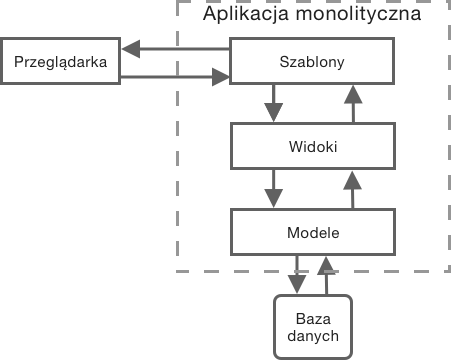
\includegraphics[width=12cm]{Rysunki/Rozdzial3/architekturaMono}
		\caption{Schemat architektury monolitycznej.}	
		\label{fig:architekturaMono}
	\end{figure}

\subsection{Mikrousługi}
Architektura mikrousług będzie zakładała, że jedna centralna aplikacja zostanie rozbita na mniejsze działające osobno. W celu porównania obu serwisów baza danych nie będzie dzielona na mniejszą, tak aby to nie zapis~i odczyt do niej był decydującym czynnikiem wskazującym na wyższość jednego~z rozwiązań, ale będzie korzystać~z różnych baz jednej usługi.

Aplikacja zarządzająca listami zadań posiadałaby cztery podstawowe moduły. Pierwszy~z nich \textbf{interfejs użytkownika}, który za pomocą dostarczanego~z przeglądarką \textit{Fetch Api}\cite{mdn} kontaktuje się~z resztą aplikacji. Użytkownik po wejściu na stronę główną przechodzi do zakładki logowania. Następnie informacje wymagane do zalogowania wpisuje~w formularz~i przesyła żądanie do usługi \textbf{użytkownicy}, zwraca ona dane użytkownika~z jego aktualnym \textit{tokenem}. Interfejs użytkownika sprawdza następnie jego poprawność~w jednostce \textit{autentykacja}\cite{Herman:2017}, gdy wszystko się zgadza klient dostaje ten sam \textit{token} z powrotem. Gdyby dany token istniał, ale jego termin ważności wygasł, to ta usługa jest odpowiedzialna za wygenerowanie nowego. Uzyskany klucz od tej pory służy do otrzymywania informacji zarezerwowanych jedynie dla zalogowanych użytkowników. Inną usługą są listy zadań, komponent ten odpowiada za zwracanie, tworzenie~i usuwanie, zadań dla poszczególnych ich właścicieli.
\begin{figure}[h!]
	\centering
		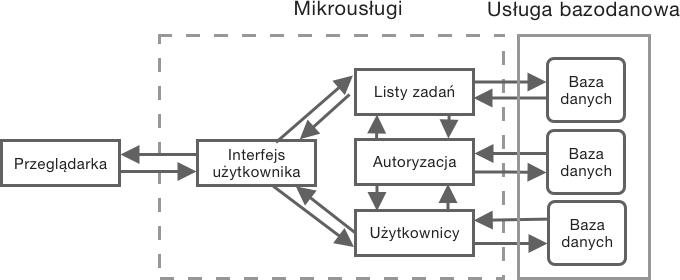
\includegraphics[width=14cm]{Rysunki/Rozdzial3/architekturaMirko.png}
		\caption{Schemat architektury mikrousług.}	
		\label{fig:architekturaMikro}
	\end{figure}

\section{Baza danych}
\label{sec:bazadanych}
Baza danych będzie posiadała dwie główne tabele: użytkownicy~i listy zdań. Będą one połączone za pomocą relacji \textit{one-to-many} w wielu \textit{frameworkach} nazywanej również kluczem obcym. Oznacza to, że jeden użytkownik będzie mógł mieć wiele zadań przypisanych do siebie, natomiast jedno zadanie będzie przypisane tylko do jednego użytkownika. Struktura ta szczegółowo została pokazana na schemacie poniżej.
\begin{figure}[h!]
	\centering
		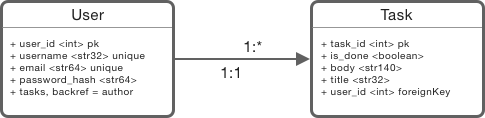
\includegraphics[width=12cm]{Rysunki/Rozdzial3/databaseSchema.png}
		\caption{Schemat bazy danych.}	
		\label{fig:schematbazydanych}
	\end{figure}
	
Jak można zauważyć na schemacie (rys.\ref{fig:schematbazydanych}), użytkownik posiada pole \textit{tasks}, które odpowiada za relację \textit{one-to-many} i tworzy referencję wsteczną\cite{Wilton:2005} dla modelu zadań~o nazwie \textit{author}, dzięki temu korzystając~z listy zadań nadal można mieć dostęp do informacji~o kliencie. Doprowadza to do potrzeby stworzenia pola \textit{user\_id} (klucza obcego) i ustanowienia relacji \textit{many-to-one} po stronie zadania.

Inną sprawą jest też, aby każdy użytkownik posiadał unikatowy \textit{username} i \textit{email}, tak żeby nie było sytuacji, w której wyciągając te informacje~z bazy danych, a następnie nimi operując nie wysłać emaila~z jakimiś wrażliwymi danymi do dwóch osób na raz. W bazie danych hasła użytkowników nie są zapisane zwykłym tekstem (ang. \textit{plain text}), ale są zatajone za pomocą funkcji haszującej (ang. \textit{hash function}). Domyślnie zestaw narzędzi \textit{Werkzeug} posiada odpowiednie metody spełniające standard \textit{PBKDF2} i wykorzystujące algorytm \textit{SHA-1} do szyfrowania haseł\cite{Ziade:2018}.

 
%=================================================================================================
\section{Wykorzystane biblioteki}
Ważne jest, aby aplikacja monolityczna, tak jaki~i te mniejsze mikrousługi oparte były~o ten sam zestaw technologii za nie odpowiedzialny. Dlatego większość wymienionych bibliotek będzie użytych~w obu projektach. W liście zostały uwzględnione tylko te główne pakiety. Wiele~z nich domyślnie instaluje mniejsze jako swoje zależności~i wypisanie ich wszystkich nie jest konieczne, aby zrozumieć działanie aplikacji. Lista najistotniejszych znajduje się poniżej:

\begin{itemize}
	\item \textit{Vue.js}\cite{vuejs}, biblioteka odpowiadająca za warstwę prezentacji.
	\item \textit{Flask}\cite{flask}, \textit{mikroframework} odpowiedzialny za usługę serwera \textit{HTTP}.
	\item \textit{Nuxt.js}\cite{nuxtjs}, framework do tworzenia progresywnych aplikacji oparty~o \textit{Vue.js}.
	\item \textit{Flask SQLAlechmy}\cite{flasksql}, system do zarządzania bazą danych~w ramach aplikacji napisanych we \textit{Flask}u. 
\end{itemize}
% TODO opisać więcej bibliotek


%=================================================================================================
\section{Analiza wymagań}
Tworzone na potrzebę pracy projekty powinny mieć zdefiniowane wymagania, tak aby jasne były konkretne ich cele do zrealizowania. Ma to zapobiec implementacji nadmiarowej ilości funkcji, a przy okazji wyszczególnić zestaw cech, które definiują projekt jako gotowy. W związku~z tym, że celem pracy jest porównanie dwóch architektur, to sam projekt nie musi działać jak pełnoprawny produkt, a jedynie posiadać wszystkie istotne elementy potrzebne do realizacji danej architektury~i możliwości porównania jej~z drugą.

\subsection{Wymagania funkcyjne}
Korzystając~z wspieranych przeglądarek internetowych (rozdział \ref{sec:przegladarki}), użytkownik powinien móc wejść na wskazany adres~i wczytać stronę główną projektu. Następnie klikając odnośnik \textit{login} na górnej belce serwisu, następuje przekierowanie do strony logowania, gdzie będzie możliwy wybór jednego~z dwóch formularzy, jeden do zalogowania już istniejącego użytkownika, a drugi do jego zarejestrowania. Po ich wypełnieniu~i przesłaniu następuje autentykacja, dzięki czemu osoba korzystające~z serwisu będzie mogła przeglądać utworzstone przez siebie zdania, tworzyć nowe~i je usuwać. Dodatkowo możliwe będzie określenie czy zadanie zostało wykonane. Powyżej listy celów będzie znajdował się przełącznik do wyświetlania zadań, które nie zostały skończone, a także tych które są gotowe. Szata graficzna strony będzie minimalistyczna, wyróżniać się będą różne rodzaje szarości. Po skończeniu korzystania~z strony użytkownik będzie mógł się~z niej wylogować, wówczas straci dostęp do listy zadań~i nie będzie mógł tworzyć nowych, ani edytować istniejących.

\subsection{Wymagania niefunkcyjne}
Istotą projektów jest sprawdzenie dwóch różnych podejść przy tworzeniu aplikacji internetowych. Ważne jest przetestowanie podstawowych funkcji, które oferują serwisy, takich jak logowanie użytkownika, tworzenie formularzy, wysyłanie zapytań: \textit{GET, POST, DELETE, UPDATE, PUT}\footnote{Podstawowe rodzaje zapytań dla standardu \textit{HTTP} \textit{REST}.} i komunikacja pomiędzy poszczególnymi komponentami serwera. Obie strony powinny posiadać również interfejs użytkownika, wraz~z skryptami~w języku \textit{JavaScript} i arkuszami styli \textit{CSS}.

Oba projekty będą wykorzystywać konteneryzację do spakowania ich~i łatwiejszego uruchomienia na maszynie programisty, prywatnym serwerze wirtualnym lub usłudze do serwowania serwisów internetowych.

\section{Środowisko programistyczne}
Obie aplikacje będą dzielić się na stronę serwerową~i warstwę prezentacji. Końcowy użytkownik do działania serwisu będzie potrzebował jedynie przeglądarki. Natomiast do uruchomienia serwera potrzebne będzie narzędzie odpowiadające za konteneryzację projektu.
 \subsection{Aplikacja serwera}
 Narzędziem wykorzystanym do konteneryzacji projektu jest \textit{Docker}, dzięki tej usłudze żadne inne zależności ani programy nie są wymagane. Należy jedynie pobrać program~z strony: \url{https://docs.docker.com/get-docker/} i~w zależności od zainstalowanego na komputerze systemu operacyjnego, odpowiednio przejść wszystkie kroki~w instalatorze.
 
 Po instalacji wystarczy, że usługa ta zostanie uruchomiona\footnote{Dla systemów~z rodziny \textit{Linux} konfiguracja jest nieco trudniejsza. Trzeba dodać jeszcze \textit{Dockera} do specjalnej grupy, aby przy każdym uruchomieniu nie używać praw administratora, \textit{sudo}. Opis procedury znajduje się na stronie \url{https://docs.docker.com/engine/install/debian/}. Dodatkowo należy stworzyć \textit{demon}, żeby narzędzie uruchamiało się przy starcie systemu, link do opisu procedury \url{https://docs.docker.com/config/daemon/systemd/}.} i~w terminalu przejść do głównego katalogu projektu, a następnie wpisać \verb|docker-compose up --build|. Komenda ta odpowiada za odnalezienie pliku \textit{docker-compose.yml}, następnie zbudowanie zadeklarowanych~w nim serwisów (przy pomocy plików \textit{Dockerfile}), a na końcu ich uruchomieniu\cite{docker}. Wówczas~w terminalu powinny pojawić się logi~z działania serwera~i odnośnikami \textit{URL} ich adresów~w przeglądarce.

\subsection{Wspierane przeglądarki}
\label{sec:przegladarki}
Projekt nie skupia się na optymalizacji go pod poszczególne przeglądarki, w szczególności te, które nie wspierają podstawowych technologii \textit{CSS}, takich jak \textit{flexbox}\cite{mdn}. W związku~z tym wsparcie nie obejmuje \textit{Windows Explorera} w wersji mniejszej niż 11, a także innych przeglądarek~w starszych wersja. Aplikacja powinna działać prawidłowo na wszystkich nowych przeglądarkach takich jak \textit{Firefox, Chrome, Opera, Microsoft Edge} i \textit{IE 11} oraz aplikacjach dostępnych dla systemu \textit{Android/iOS}.
